% Figure from MATH 591 notes, section 12. Compile with the notes preamble.
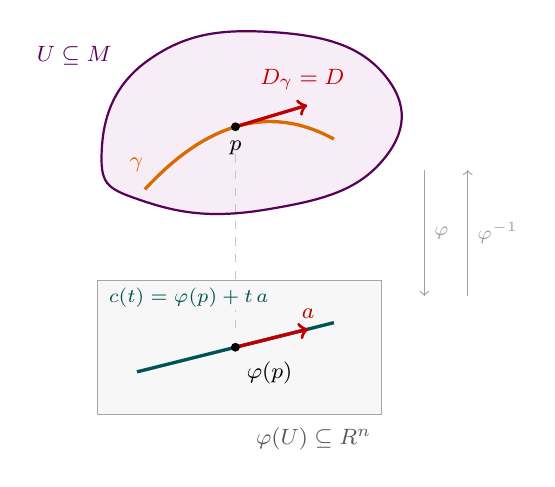
\begin{tikzpicture}
\draw[violet!70!black,fill=violet!7,thick] plot[smooth cycle,tension=0.8] coordinates {(0.9,3.05) (1.5,4.25) (3.1,4.6) (4.5,4.05) (4.45,2.95) (3.0,2.35) (1.45,2.45)};
\draw[orange!85!black,very thick] (1.450,2.605) -- (1.480,2.638) -- (1.511,2.670) -- (1.541,2.701) -- (1.572,2.732) -- (1.602,2.762) -- (1.632,2.791) -- (1.663,2.820) -- (1.693,2.848) -- (1.723,2.876) -- (1.754,2.903) -- (1.784,2.929) -- (1.815,2.955) -- (1.845,2.980) -- (1.875,3.004) -- (1.906,3.028) -- (1.936,3.051) -- (1.966,3.073) -- (1.997,3.095) -- (2.027,3.117) -- (2.058,3.137) -- (2.088,3.157) -- (2.118,3.177) -- (2.149,3.195) -- (2.179,3.214) -- (2.209,3.231) -- (2.240,3.248) -- (2.270,3.264) -- (2.301,3.280) -- (2.331,3.295) -- (2.361,3.309) -- (2.392,3.323) -- (2.422,3.336) -- (2.453,3.348) -- (2.483,3.360) -- (2.513,3.371) -- (2.544,3.382) -- (2.574,3.392) -- (2.604,3.401) -- (2.635,3.410) -- (2.665,3.418) -- (2.696,3.426) -- (2.726,3.432) -- (2.756,3.439) -- (2.787,3.444) -- (2.817,3.449) -- (2.847,3.453) -- (2.878,3.457) -- (2.908,3.460) -- (2.939,3.463) -- (2.969,3.464) -- (2.999,3.466) -- (3.030,3.466) -- (3.060,3.466) -- (3.091,3.465) -- (3.121,3.464) -- (3.151,3.462) -- (3.182,3.459) -- (3.212,3.456) -- (3.242,3.452) -- (3.273,3.448) -- (3.303,3.443) -- (3.334,3.437) -- (3.364,3.431) -- (3.394,3.424) -- (3.425,3.416) -- (3.455,3.408) -- (3.485,3.399) -- (3.516,3.390) -- (3.546,3.379) -- (3.577,3.369) -- (3.607,3.357) -- (3.637,3.345) -- (3.668,3.333) -- (3.698,3.319) -- (3.728,3.306) -- (3.759,3.291) -- (3.789,3.276) -- (3.820,3.260) -- (3.850,3.244);
\draw[red!75!black,->,very thick] (2.600,3.400) -- (3.510,3.673);
\node[red!75!black,font=\footnotesize,anchor=south] at (3.45,3.74) {$D_\gamma = D$};
\fill (2.600,3.400) circle (1.6pt); \node[font=\footnotesize,anchor=north] at (2.600,3.340) {$p$};
\node[orange!85!black,font=\footnotesize,anchor=south east] at (1.550,2.710) {$\gamma$};
\node[violet!70!black,font=\footnotesize,anchor=east] at (1.15,4.3) {$U \subseteq M$};
\draw[gray!70,fill=gray!6] (0.85,-0.25) rectangle (4.45,1.45);
\draw[gray!45,dashed] (2.600,3.050) -- (2.600,0.850);
\draw[teal!65!black,very thick] (1.350,0.287) -- (3.850,0.912);
\draw[red!75!black,->,very thick] (2.600,0.600) -- (3.522,0.830) node[anchor=south,font=\footnotesize]{$a$};
\fill (2.600,0.600) circle (1.6pt); \node[font=\footnotesize,anchor=north west] at (2.620,0.540) {$\varphi(p)$};
\node[teal!65!black,font=\scriptsize,anchor=north west,fill=gray!6,inner sep=1pt] at (0.95,1.4) {$c(t) = \varphi(p) + t\,a$};
\node[gray!70!black,font=\footnotesize,anchor=north east] at (4.45,-0.3) {$\varphi(U) \subseteq \mathbb{R}^n$};
\draw[->,gray!75] (5.0,2.85) -- node[right,font=\scriptsize]{$\varphi$} (5.0,1.25);
\draw[->,gray!75] (5.55,1.25) -- node[right,font=\scriptsize]{$\varphi^{-1}$} (5.55,2.85);
\end{tikzpicture}
